% coding:utf-8

\section{Elektrischer Strom aus Wärme}

% \subsection{Aufbau}
% \begin{frame}

% \end{frame}

% \subsection{Modulation}
% \begin{frame}
% \end{frame}

% \subsection{Kalibrierung}
% \begin{frame}
%   \begin{figure}
%     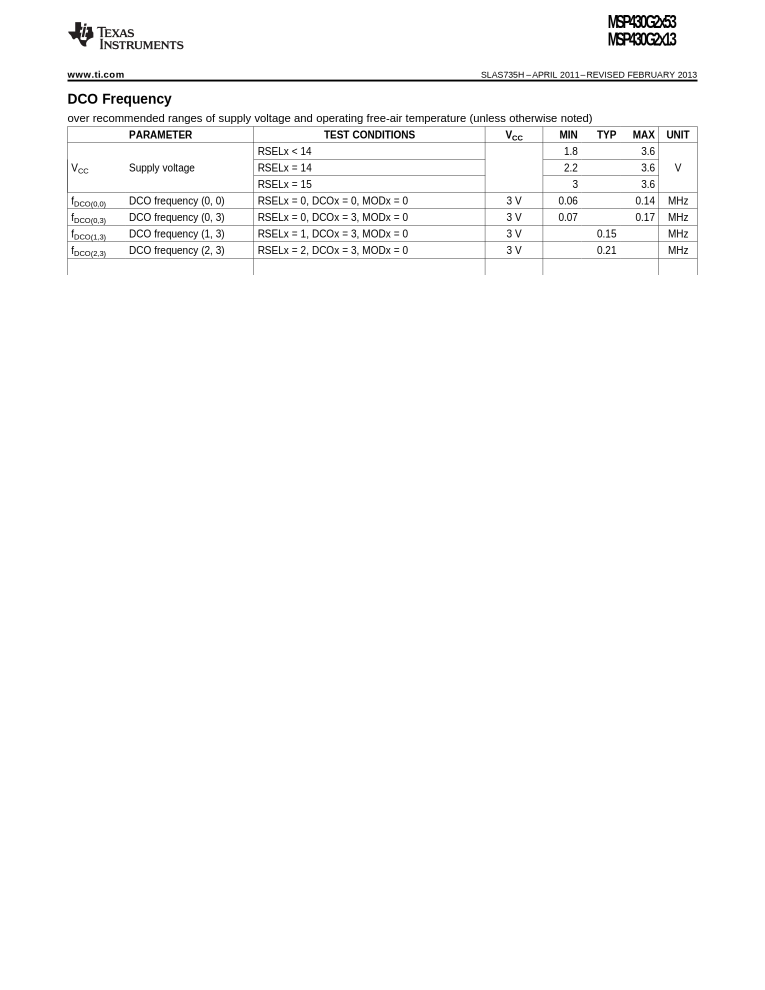
\includegraphics[width=1.0\columnwidth]{fig/ti_ds_dco_freq.pdf}
%     \caption{Auszug aus dem Datenblatt des MSP430G2553}
%   \end{figure}
% \end{frame}
\subsection{Wärmeenergie $\Rightarrow$ Elektrische Energie}
\begin{frame}
\begin{block}{Nachteile}
  \begin{itemize}
    \item Geringer Wirkungsgrad\\
          Bisher $\approx$ 10 \%
  \end{itemize}
\end{block}
\begin{block}{Potential}
  \begin{itemize}
    \item Nutzung von Abwärme
    \item Energieerzeugung in der Raumfahrt
  \end{itemize}
\end{block}
\end{frame}

\subsection{Thermoelektrische Generatoren}
\begin{frame}
\begin{block}{Funktion}
  \begin{itemize}
    \item Halbleiter
    \item Temperatur $\Rightarrow$ Thermoelektrische Spannung
  \end{itemize}
\end{block}
\begin{block}{Fortschritt}
  \begin{itemize}
    \item geringe Wärmelaitfähigkeit
    \item neues Herstellungsverfahren
    \item neue Materialien
  \end{itemize}
  \begin{itemize}
    \item $\Rightarrow$ Wirkungsgrad bis 20 \%
  \end{itemize}
\end{block}
\end{frame}